\documentclass[12pt,a4paper]{scrartcl}

\usepackage[a4paper, left=2cm, right=2cm, bottom=1cm, top=1cm, includeheadfoot]{geometry}
\usepackage[ngerman]{babel}
\usepackage[utf8]{inputenc} % comment this if you uncomment utf8x
%\usepackage[utf8x]{inputenc} % uncomment this if there are problems with 'ä', 'ü', 'ö'
\usepackage{ucs}
\usepackage[usenames,dvipsnames]{xcolor}
\usepackage[fleqn]{amsmath}
\usepackage{amsfonts}
\usepackage{amssymb}
\usepackage{color}
\usepackage{listings}
\usepackage{hyperref}
\usepackage{amsfonts}
\usepackage{listings}
\usepackage{scrpage2}
\usepackage{graphicx}
\usepackage{pdfpages}
\usepackage{mathtools}
\usepackage{multirow}
\usepackage{float}
\usepackage{matlab-prettifier}


\definecolor{mygray}{rgb}{0.9,0.9,0.9}
\lstset{language=[Visual]Basic, morekeywords={param, local}}


\lstset{
   literate={ö}{{\"o}}1
           {ä}{{\"a}}1
           {ü}{{\"u}}1
           {ß}{{\ss}}1
           {é}{{\'e}}1,
   inputencoding=ansinew,
   extendedchars=true,
   basicstyle=\scriptsize\ttfamily,
   numberstyle=\scriptsize,
   breaklines=true,
   tabsize=4,
   numbersep=5pt
}
\lstdefinestyle{customcpp}{
   language=C++,
   backgroundcolor=\color{mygray},
   numbers=left,
   keywordstyle=\color{blue}\bfseries,
   stringstyle=\color{BrickRed}\ttfamily,
   commentstyle=\color{OliveGreen}\ttfamily,
   showspaces=false,
   showstringspaces=false,
   showtabs=false
}
\lstdefinestyle{customoutput}{
   backgroundcolor=\color{mygray},
   numbers=none,
   showspaces=false,
   showtabs=false
}

\newcommand{\sourceCode}[1]{\lstinputlisting[style=customcpp]{#1}}
\begin{document}

\title{SCD5 - Matlab - Übung 4}
\date{\today}
\author{Daniel Klepatsch \and Thomas Reisinger}
        
\maketitle

\newpage

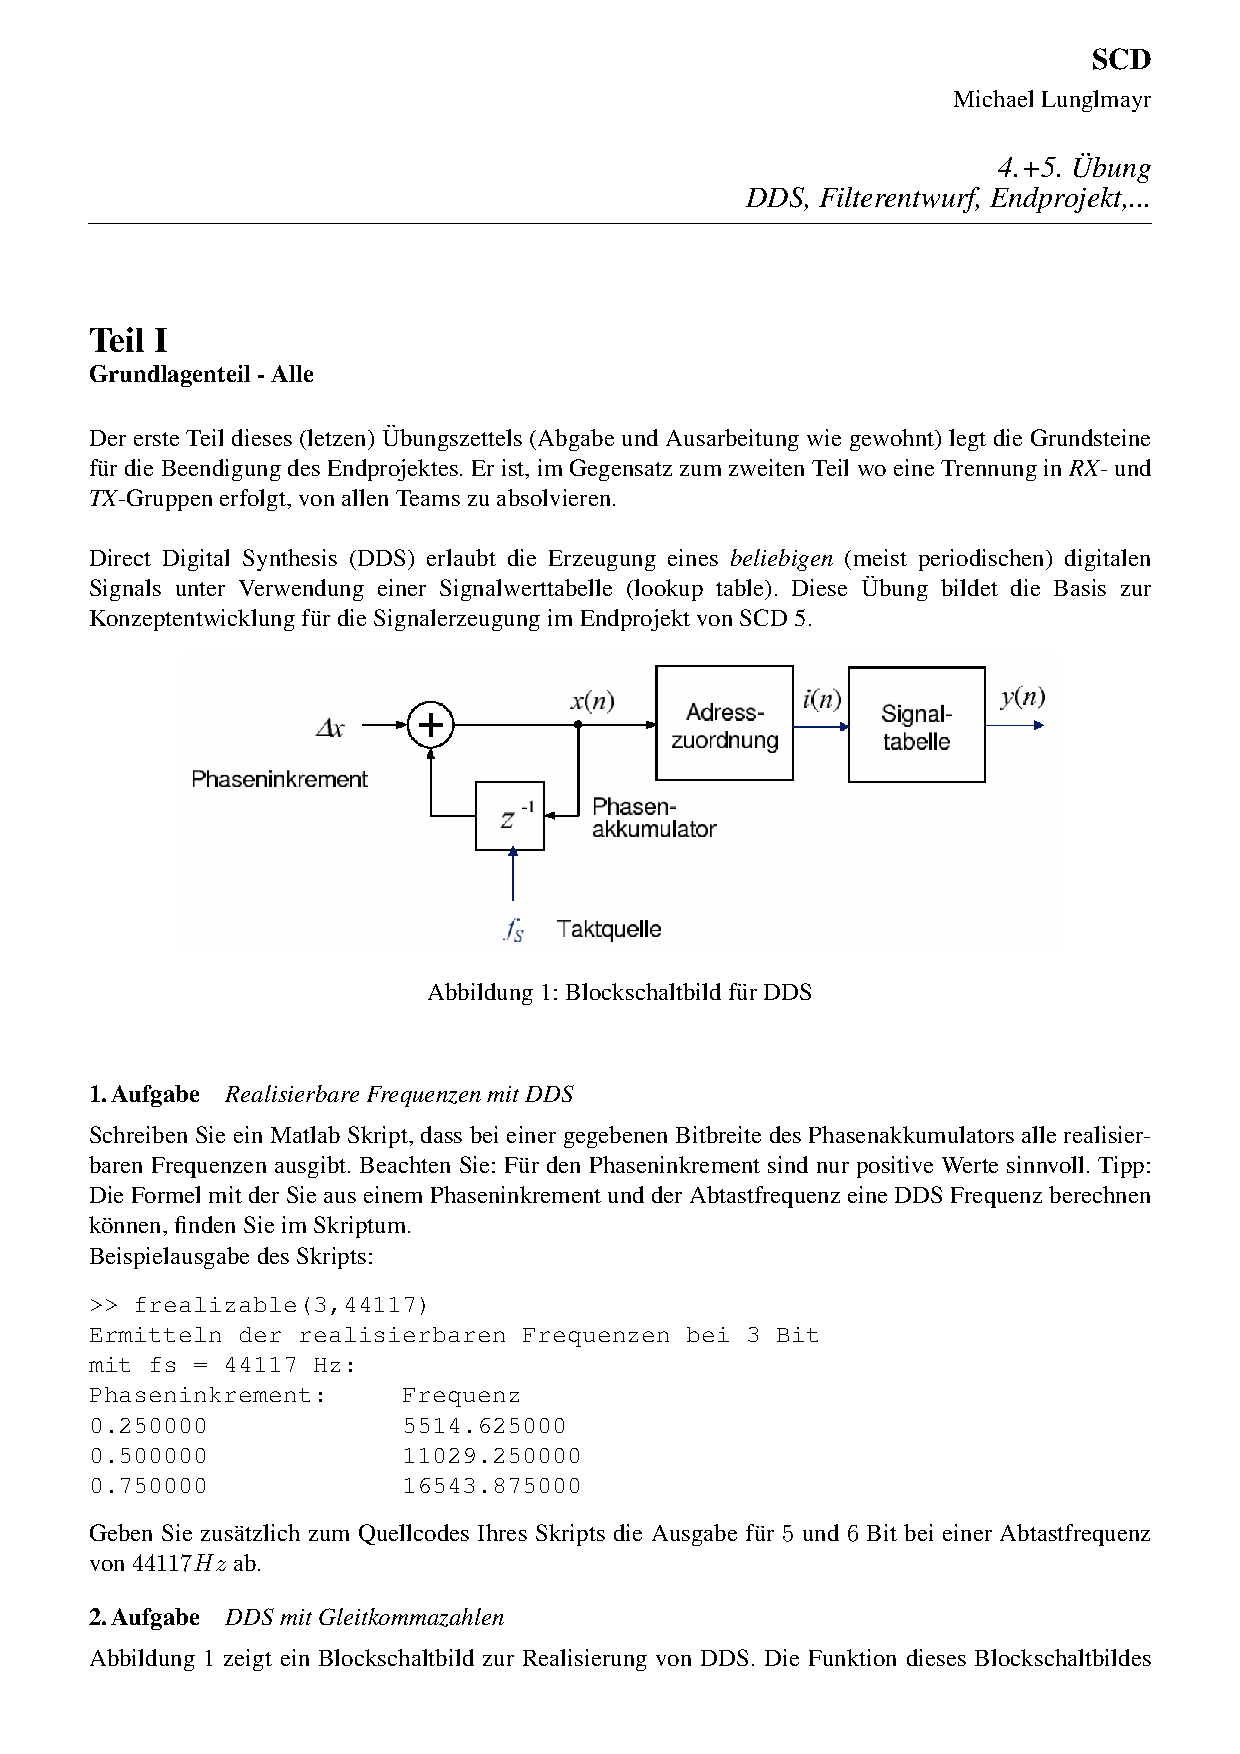
\includepdf[pages=-]{../SCD_UE04_Deckblatt.pdf}

\tableofcontents

\newpage

\section{Aufgabe 1 - Realisierbare Frequenzen mit DDS}

\subsection{Matlab-Skript}

\sourceCode{../../../workspace/frealizable.m}

\subsection{Ausgabe für 5 Bit}

\sourceCode{../bsp1_5_Bit.txt}

\newpage

\subsection{Ausgabe für 6 Bit}

\sourceCode{../bsp1_6_Bit.txt}

\newpage

\section{Aufgabe 2 - DDS mit Gleitkommazahlen}

\subsection{Matlab-Skript}

\sourceCode{../../../workspace/scd4_2_start.m}

\newpage

\subsection{Vergleich der Signale}

\begin{center}
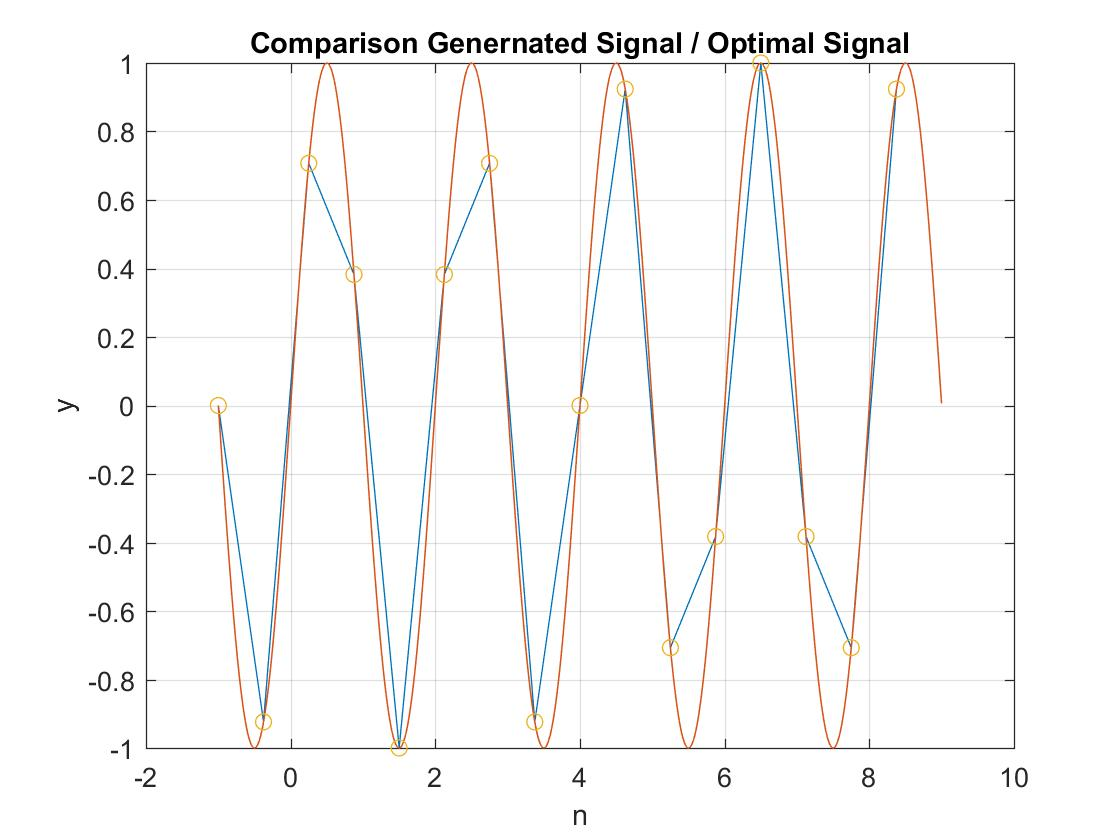
\includegraphics[scale=0.35]{../fig4_2_1_comparison.jpg}
\end{center}

\subsection{Spektrum des generierten Signals}

\begin{center}
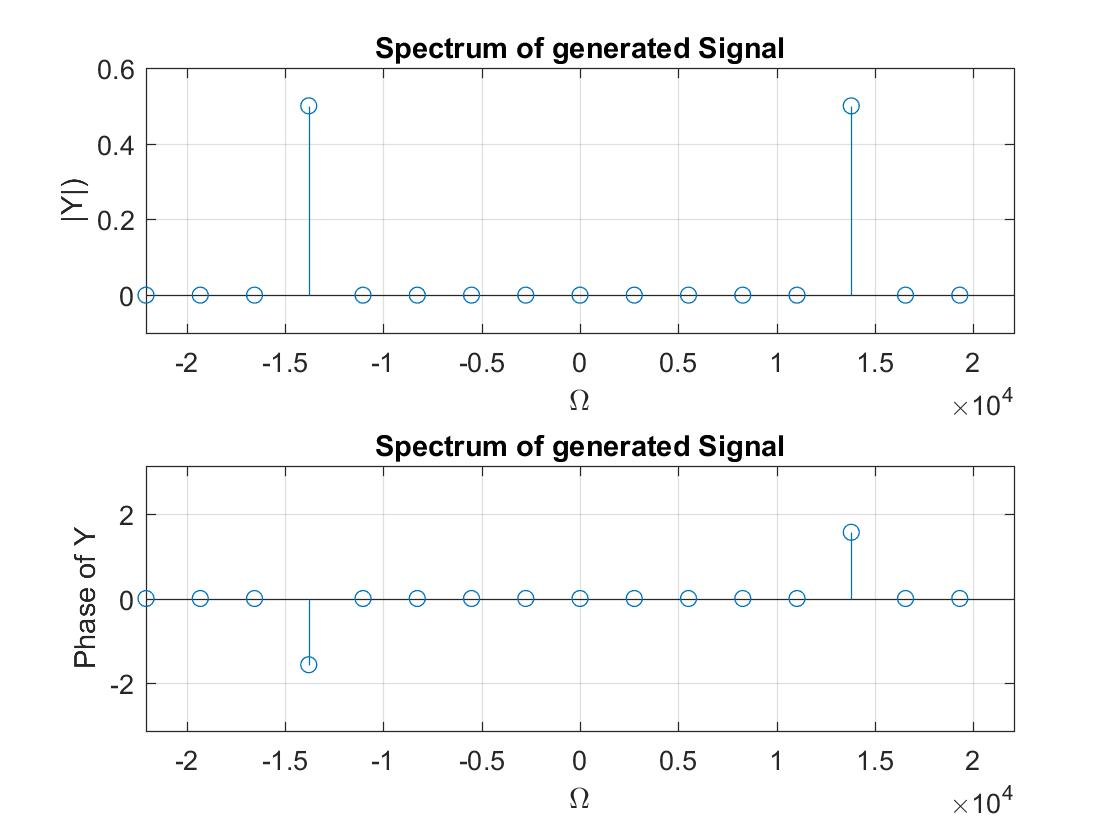
\includegraphics[scale=0.35]{../fig4_2_2_spectrum.jpg}
\end{center}

\newpage

\subsection{Fragen}
\begin{itemize}
\item{a)} Es wurde eine Frequenz von 13786,5625Hz erzeugt, dies entspricht einer Abweichung von 1,5482\% zu 14kHz.
\item{b)} Für das gegebene Beispiel werden 5 Perioden benötigt.
\item{c)} Die resultierende Frequenz stimmt mit der in Aufgabe 1 berechneten Frequenz überein.
\item{d)} Je mehr Werte in der Tabelle stehen, desto genauer wird der Sinus und desto weniger Störungen sind im Spektrum zu sehen.
\item{e)} Es werden 16 Signalwerte benötigt, bis sich das Signal wiederholt.
\item{f)} Die DFT benötigt zur Analyse ein periodisches Signal, tritt keine Periode auf, so entsteht ein Sprung, dieser ist im Spektrum erkennbar.
\end{itemize}

\newpage

\section{Aufgabe 3 - DDS mit Interpolation}

\subsection{Matlab-Skript}

\sourceCode{../../../workspace/scd4_3_start.m}

\newpage

\subsection{Plots}

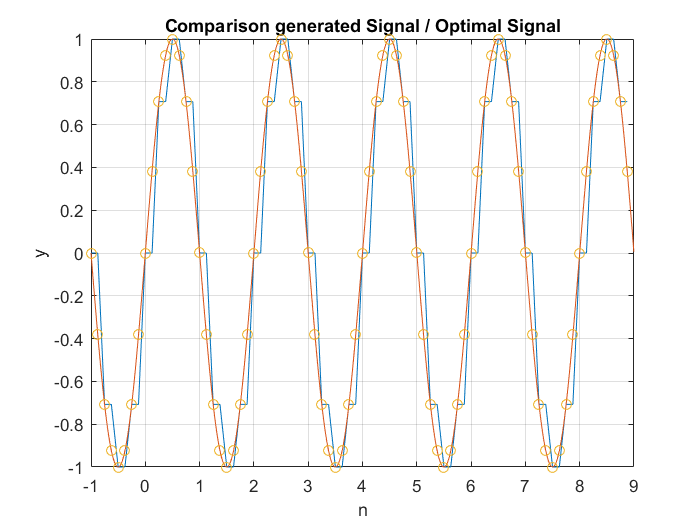
\includegraphics[scale=0.45]{../ue04_b3_1.png}
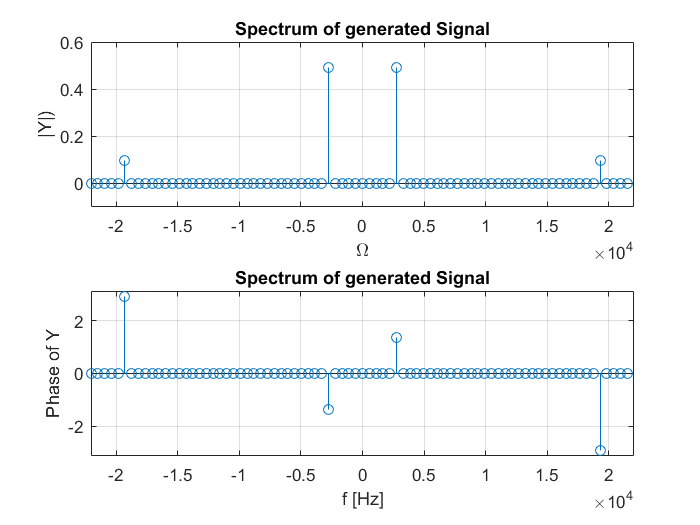
\includegraphics[scale=0.45]{../ue04_b3_2.png}
\\
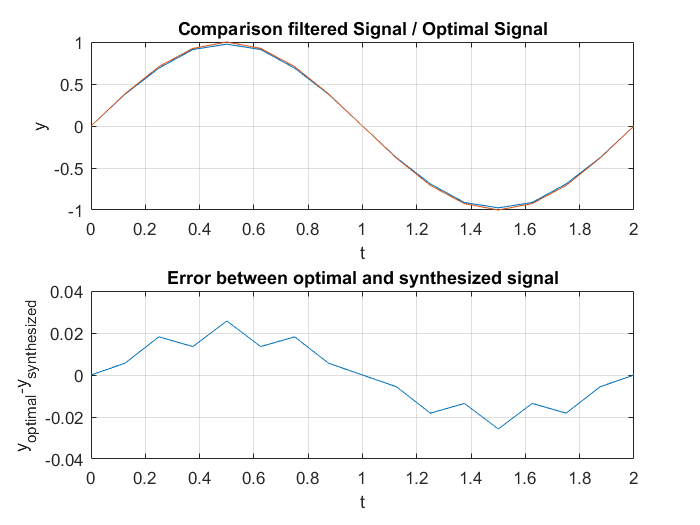
\includegraphics[scale=0.45]{../ue04_b3_3.png}
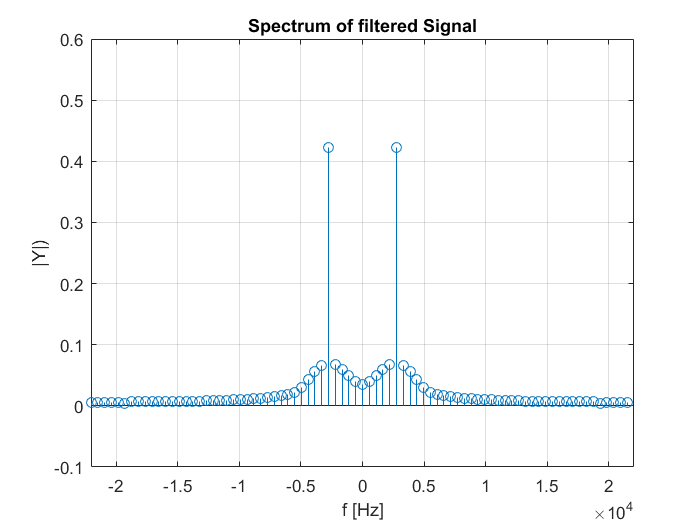
\includegraphics[scale=0.45]{../ue04_b3_4.png}

\subsection{Fragen}
\begin{itemize}
\item{a)} gemessene Frequenz: 2757.3Hz
\item{b)} Neben der erreichten Frequenz treten weitere Frequenzen auf.
\item{c)} omegapass muss größer als die Frequenz des Signals sein, damit diese nicht weggefiltert wird. omegastop wurde so gewählt, dass die Amplitude des Signals maximiert ist. Die Rippel im Durchlass- und Sperr-bereich müssen kleiner, als das halbe Phaseninkrement sein, um Rundungsfehler zu vermeiden. Gewählt wurde 1/4 des Phaseninkrements.
\item{d)} Der maximale Fehler beträgt 2.5699%.
\item{e)} Es wurde das vorliegende Ergebnis erwartet.
\item{f)} Den Tiefpass könnte man sich ersparen, wenn mehr Werte in der Sinustabelle vorliegen würden.
\end{itemize}

\newpage

\section{Aufgabe 4 - Filterentwurf mit fdatool}

\subsection{Plot}

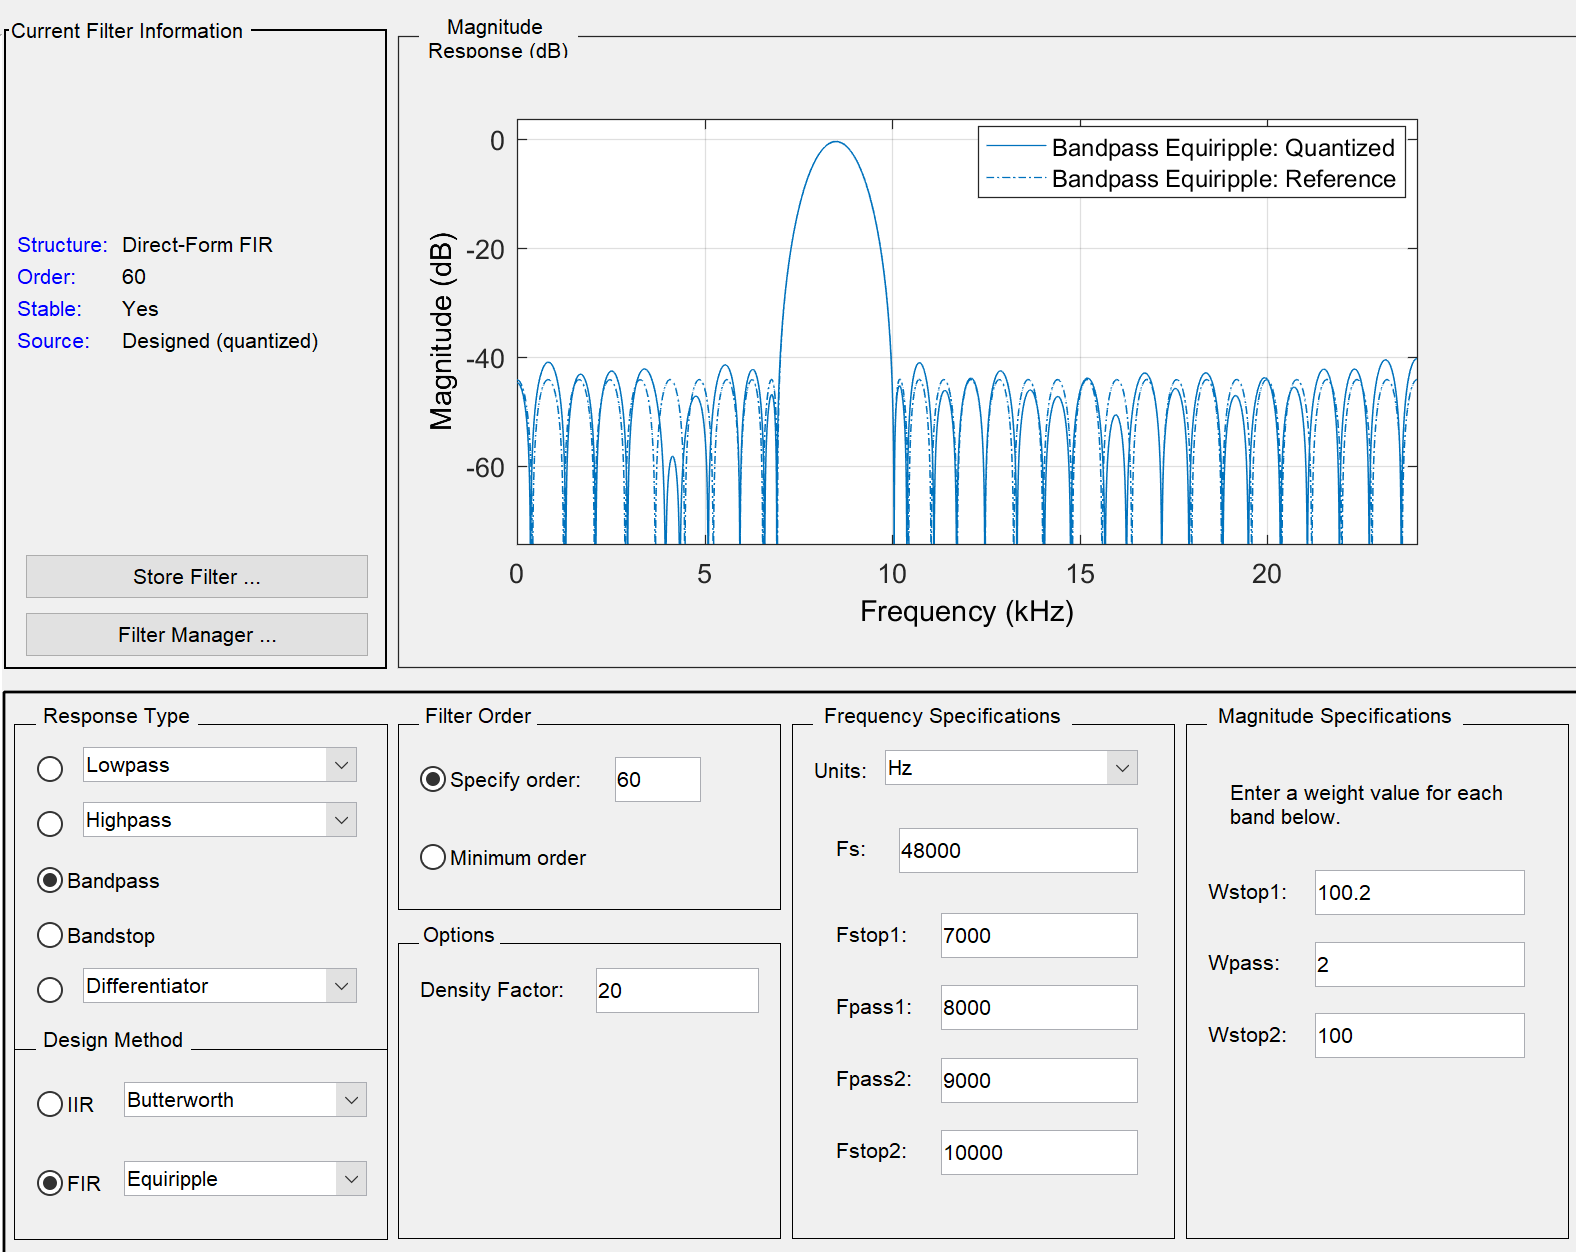
\includegraphics[scale=0.8]{../plot4_4.png}

\subsection{Fragen}

\begin{itemize}
\item{a)} Es wurden 60 Koeffizienten verwendet.
\item{b)} Für die verwendeten 60 Koeffizienten wurden 11 Bit benötigt um das Entwurfsschema einhalten zu können.
\end{itemize}

\newpage

\end{document}